\chapter{Introduction}
\label{cha:introduction}

% Most enterprise tools nowadays support multiple companies as users. And of course for organization each company needs to have their own sepparate space to work in


% The focus of this thesis, is to propose and implement a multi-tenant feature for Management System of PROCEED.
% PROCEED(PROCess EnginE in a Distributed environment) is a BPMN process engine.
% BPMN is an abstraction used to model business logic. 
% PROCEED has a Management System, where users can manage their BPMN models.
% Environments allow users to manage everything that PROCEED offers with a layer of sepparation, meaning that, the contents of each environments, are separate to all other environments.

% Nowadays cloud applications have become very popular in professional settings.
% Cloud applications are those, which are served and accessed over the internet, they offer many benefits:

In today's digital age, businesses heavily rely on cloud applications, software tools that
are accessed and run entirely over the internet. Cloud applications offer many advantages:

\begin{itemize}
    \item Accessibility: They can be accessed anywhere from anywhere with an internet connection.
    \item Cost-Efficient: Most cloud applications offer a subscription model, where you have to pay a monthly price, instead of paying for the whole software upfront.
    \item Collaboration: Typically, collaboration is easier since everything can be found
      in one place, instead of having to send files back and forth.
    \item Data safety: All files are stored by the application in the cloud, and they don't
      have to be stored in the user's device, which could be lost, stolen or damaged.
      % users don't have to implement their own data storage solutions,
      % which may be insecure.
    \item Device agnostic: many cloud applications can be accessed through different device types.  
    \item No IT overhead: users don't have to setup the application on their own, which would require technical knowledge.
\end{itemize}

\begin{figure}[H]
    \centering
    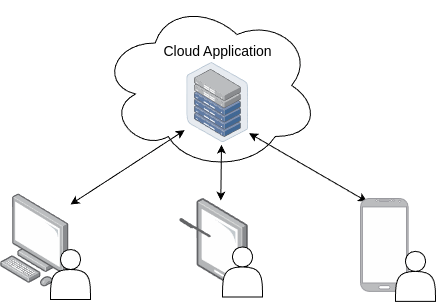
\includegraphics[scale=0.35]{images/basic-cloud-services.drawio.png}
    \caption{Cloud Application.}
    \label{fig:cloud-applications}
\end{figure}

% A key selling point of these, is that companies don't have to do any technical work setting the software up, they can pay for a subscription and start using the tool right away, either through a browser or by installing an executable on their computer.
% A very important technical aspect for such tools, that enables the ease of use, is the ability to support multiple companies using them at once.

% Most of these benefits only apply if all users interact with the same cloud application.
% This means that the users interact with what appears to them to be a single application
% This is called multi-tenancy, and it is implemented by most popular cloud applications, e.g. by Teams, Slack, Asana, and many more.
% A tenant can be seen as an entity that uses the application, which can be either a single user or an organization made up of many users.

One very common feature that makes these benefits possible is called "multi-tenancy".
Multi-tenancy is a software architecture in which one single instance of an application
can be used by many different users or organizations at the same time. 
Without multi-tenancy, each user or organization would need to run the application on
their own servers or computers, 
largely negating the numerous benefits listed earlier.

% means that many different users or organizations can use the same cloud application at the same
% time, even though it looks like they each have their own private version.

% NOTE: maybe take this out
Think of it like a big apartment building. Each tenant (user or organization) has their
own private space (their assets), but they're all using the same building (the
cloud application).

Many popular cloud applications use this approach. For example, when you use Microsoft Teams,
Slack, or Asana, you're sharing the application with many other companies, but you only
see and interact with your own team.

\begin{figure}[H]
    \centering
    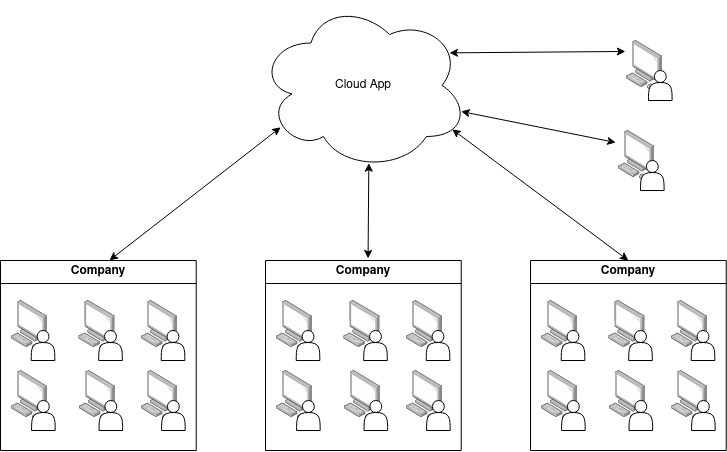
\includegraphics[scale=0.45]{images/mt-cloud-services.png}
    \caption{Multi tenancy in cloud applications.}
    \vspace{-1em} % Negative value to remove space
    \label{fig:multi-tenant=cloud-applications}
\end{figure}

PROCEED (short for PROCess EnginE in a Distributed environment) %is a cloud application,
is a decentralized Business Process Management System.
PROCEED uses BPMN at its core to model and execute business processes.
%For readers unfamiliar with BPMN, 
%it can be thought of as a powerful flowchart that can be used to describe any conceivable process.
BPMN (Business Process Model and Notation) is a standardized graphical notation used for documenting business processes.
BPMN is typically used inside of organizations to illustrate sequences of tasks,
decision points, and interactions within various business processes, providing a standardized visual representation.

PROCEED offers two products:
\begin{itemize}
    \item Distributed Process Engine (DPE for short): the DPEs execute bpmn processes in a distributed fashion.
    \item Management System (MS for short): the MS is a cloud application that gives users
      a graphical interface to work on their BPMN processes and deploy these to the DPEs.
\end{itemize}

\begin{figure}[H]
    \centering
    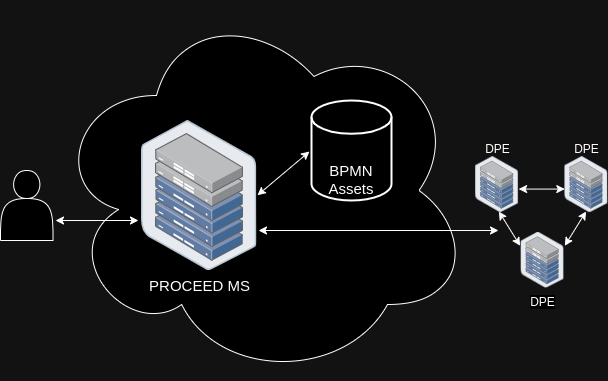
\includegraphics[scale=0.45]{images/quick-ms-overview.drawio.png}
    \caption{Overview of PROCEED.}
    \label{fig:proceed-overview}
    \vspace{-1em} % Negative value to remove space
\end{figure}

%Throughout this thesis we'll refer to any information that a user can access as an asset.
%Also all actions that a user can perform in the PROCEED Management System, are viewed as an action performed on an asset.

%The PROCEED Management system encompasses various asset types, which can be categorized as follows:
%\begin{enumerate}
%    \item BPMN models: Processes, Projects, and Templates are assets that can be created in PROCEED, that fall into the category of BPMN models.
%    Although each one of them stores slightly different information and carries a distinct semantic meanings, they all have BPMN at their core.
%    \item Execution related assets: Tasklist, Executions and Machines are all assets related to the execution of a BPMN model.
%end{enumerate}

Currently the MS lacks full multi-tenancy support, it only supports individual users and
doesn't fully support organizations.
For organizations to be supported, members of the organization need to be able to have a
shared workspace, where they can work on the same assets. 
This could technically achieved if members of the organization shared all assets with
each other.
However, PROCEED only supports universal sharing, meaning that all users would be able to
see the shared assets.
Furthermore, even if it was possible to share assets only to a group of users, it would be
very cumbersome and error-prone.
% This means that organizations, where multiple people work together are not supported by the
% MS.
% For this reason, it presents many difficulties for organizations, as there is no convenient way for multiple members of the organization to work together on assets in the MS.
% For this reason, the MS is not suitable for organizations, as there is no convenient way
% for multiple members of an organization to work together.
% Furthermore, any admin user in the MS has the right to view and modify every asset, which presents privacy risks for organizations.
% The only somewhat viable option for organizations to use PROCEED, is to run the server
% code of the MS on their own computers, which renders most benefits of cloud applications void.
%This is because all assets are stored in a central database without a good way to isolate them from other tenants.
%The only information that BPMN related assets are stored with, that helps towards isolating them from other tenants is the owner and a set of labels.
For this reason, this thesis implements multi-tenant functionality into the PROCEED MS by introducing the concept of Environments. 

Each tenant will be able to work in their own isolated environment, which lives in a central instance of the Management System. 
Each account will automatically have its own Environment allowing users to work on
personal projects. 
Organizations will be able to create environments where multiple members can work together.

\begin{figure}[H]
    \centering
    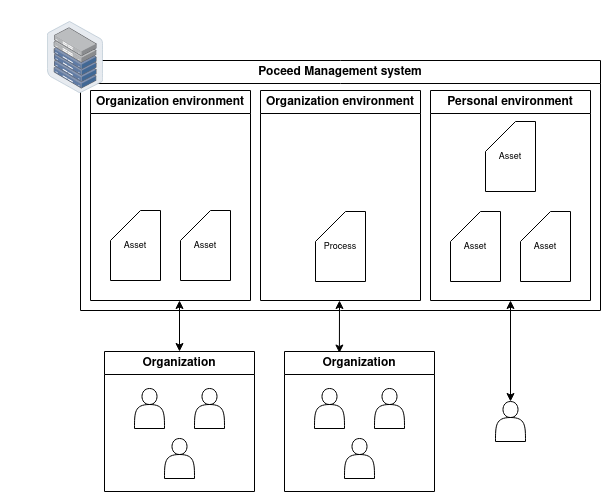
\includegraphics[scale=0.45]{images/proceed-workspaces-v2.drawio.png}
    \caption{Environments in PROCEED.}
    \label{fig:proceed-envitonments-overview}
\end{figure}
Additionally, environments will include a folder structure to improve the organization of
assets.
Currently the MS only provides labels for organizing assets.
Assets can be labeled with one or more labels, which can be used to filter assets. 
Users cannot add, delete nor modify these labels.
Folders will provide more flexibility than labels.

% These labels symbolize, what department the process belongs to. 

%Access to assets in the MS is restricted through roles,
%so that one of three scenarios can happen to a user:
%
%\begin{itemize}
%    \item The user doesn't permissions to see assets.
%    \item The user has permission to view assets, but isn't an admin. In case, the user would only be able to see his own assets.
%    \item The user is an admin and can see all assets.
%\end{itemize}
%
%This low level of granularity makes the PROCEED Management System unsuitable hosting multiple tenants, since all their assets would be stored in the same fashion, and the only way for users to see assets that weren't created by them, would be to grant them the admin role.
%Granting users the admin role, would in turn mean that they would be able to see all BPMN Assets, which poses privacy concerns for tenants, since other tenants could potentially access their assets.

%When it comes to Execution related assets, Machines and Executions also have similar problems to BPMN assets, since these need to be private for each company.

%This makes it so, that if more than one tenant wants to use PROCEED they're left with few options:
%
%\begin{itemize}
%\end{itemize}
%Each company would have to spin up their own self hosted version of PROCEED.
%
%Both of these options have considerable downsides. 
%No separation between companies is a hindrance to privacy and each company having to spin up an instance of PROCEED is a big barrier to entry.
%This makes it very hard to scale PROCEED to be able to be comfortably used by multiple companies.
%
%\begin{figure}[H]
%    \centering
%    \includegraphics[scale=0.5]{images/PROCEED-no-Environments.drawio.png}
%    \caption{PROCEED Management System with no multi-tenant support.}
%    \label{fig:PROCEED-no-Environments}
%\end{figure}


% Research questions
\chapter{Research Questions}
\label{cha:researchquestions}

\begin{enumerate}
% Data Modeling and Architecture

\item Environment Representation: How can we model environments within the existing PROCEED database schema to ensure data integrity, isolation, and efficient access? 

\item Asset-Environment Association: How can we associate assets with their respective environments while maintaining a clear and consistent data model?

\item Folder Hierarchy: What data structure (e.g., tree, graph, nested sets) is best suited for representing folder hierarchies within environments? How can we efficiently store and query this structure in the database?

% Roles and Permissions

\item How can we extend the existing PROCEED role system to incorporate
environment-specific permissions? 

\item How can we apply different permissions to assets based on what folder they are
  stored in?

\item What mechanisms are needed to ensure that role-based access control is consistently enforced?

\item How can the frontend user interface dynamically adapt to a user's roles and permissions within different environments?

% Usability and Developer Experience

\item What user interface elements and interaction patterns are most effective for navigating and managing folders and environments?

\item What software abstractions (e.g., classes, interfaces, functions) can we create to simplify the process of identifying and managing a user's environment in the backend code? 

\item How can we minimize the impact on existing code while ensuring seamless integration?

% Additional Considerations

Performance and Scalability: How will the addition of environments impact the performance and scalability of the PROCEED Management System? What optimizations can be made to ensure that the system remains responsive and efficient even with a large number of users and environments?
Migration Strategies: How can we seamlessly migrate existing PROCEED data and users into the new environment-based structure? What strategies can we employ to minimize disruption during the transition?
Security: What additional security measures are needed to protect data within environments? How can we prevent unauthorized access to environments and their assets?
\end{enumerate}

% Task List

\chapter{Task List}
\label{cha:tasklist}

% private environment
% Functional / non functional
% can / must / should 

\newlist{myEnumerate}{enumerate}{5}
\setlist[myEnumerate,1]{label=(\arabic*)}
\setlist[myEnumerate,2]{label=(\Roman*)}
\setlist[myEnumerate,3]{label=(\Alph*)}
\setlist[myEnumerate,4]{label=(\roman*)}
\setlist[myEnumerate,5]{label=(\alph*)}

\begin{myEnumerate}
  \item Functional
    \begin{myEnumerate}
      \item The MS has to support two types of environments: personal and organization environments.
        \begin{myEnumerate}
          \item Every asset in the MS must be stored in one and only one environment.

          \item Assets stored in one environment can only be accessed by members of that
            environment.

          \item Every user has to have a personal environment, of which only he can be a member.

            %NOTE: im talking about roles here, maybe should go somewhere else
          \item Organization environments must be able to have multiple members and roles that control what each member can do.

          \item Environments must have a folder system to store assets.
            \begin{myEnumerate}
              \item Find a suitable abstraction to represent folders in a database.

              \item Ensure privacy between environments.

                % escribir aca ya que tiene que haber herencia
                % reescribir should be modified no es tan fuerte/
                % likely redundant

              \item The MS's preexisting role system must be adapted to fit environments:
                The proceed management system already has a role system in place to manage user's access to resources, these roles need to be modified for them to work with environments.
                \begin{myEnumerate}
                  \item Ensure roles are always enforced in the backend.
                  \item The frontend UI must adapt to a user's roles, by only showing options that the user has permission to do.
                \end{myEnumerate}
                depending on the folder the asset is in.
            \end{myEnumerate}

        \end{myEnumerate}

        % NOTE: replace concurrently with eaesier word
      \item The MS must be able to hold multiple environments and let users access them concurrently.

        %NOTE: maybe carry out actions no the best frasing
      \item Users must be able to be members of multiple environments and carry out actions in each one of them.


    \end{myEnumerate}

  \item Non functional
    \begin{myEnumerate}
      \item keep changes to the existing codebase to a minimum.

      \item The same data structure should be used for both personal and organization environments.

        % \item The implentation shoudln't be repetitive, the same functional components should be used for both personal and organization environments.

      \item The user interface for navigating and managing folders and environments should
        be intuitive and easy to use.

      \item Prioritize developer experience by creating clear abstractions and APIs.
        \begin{myEnumerate}
          \item Create simple abstractions for the backend code of the MS, that allow to acknowledge a user's environment with minimal effort.
          \item Create a simple abstraction for the frontend, that facilitates adapting
            the Interface for each.
        \end{myEnumerate}

      % \item Environments should be easy to create, manage and delete.
      %   \begin{myEnumerate}
      %     \item The frontend should provide intuitive interfaces for creating and deleting organization environments.
      %       // not functional
      %     \item Provide well documented APIs to create, manage and delete environments both for the frontend and the backend.
      %       needs more description. ldap
      %     \item Environments should provide the option to import an existing user database.
      %   \end{myEnumerate}
    \end{myEnumerate}

\end{myEnumerate}


%---------------- 
% old

% \begin{enumerate}
% \item The same data structure should be used to represent personal and organization environments.
% \begin{enumerate}
        % \item Personal and organization environments should have a near identical structure.
        % kann man falsch verstehen umschreiben
        % \item Most of the backend and frontend code should work the same, regardless of if it is dealing with a personal or an organization environment.
    % \end{enumerate}

    % not functional - keine stichpunkte  - : 2 points in one paragraph

% \end{enumerate}

% The introduction of "environments" within this system is a pivotal enhancement. These environments serve as distinct, isolated spaces, ensuring that the contents and operations within each environment remain entirely separate from those in all other environments. This separation offers users the capability to manage various aspects of PROCEED's functionality while maintaining data and process integrity within their designated environment. This thesis explores the design, implementation, and implications of the multi-tenant feature within the Management System of Proceed, contributing to a more versatile and secure user experience.
